\section{Simulaciones}
    
    A continuación, se hará uso del siguiente código para poder hacer los cálculos adecuados para el análisis de la simulación antes mencionada en la sección \ref{sec:propuesta}. 

    \subsection{Código en Python para la simulación de pérdidas resistivas}

        %\lstinputlisting[
        %  language=Python,
        %  basicstyle=\ttfamily\small,
         % caption={Código Python para la simulación de pérdidas en el conductor},
          %label={lst:sim_perdidas}
        %]{code/sim_perdidas.py}
    

    De acuerdo con los cálculos obtenidos del código \ref{lst:sim_perdidas}, los valores de cada parámetro y, la gráfica se mostraran a continuación, de esta manera poder analizar los resultados obtenidos de la simulación realizada.

        \begin{figure}[H]
            \centering
            \setcounter{figure}{0}
            \renewcommand{\figurename}{Gráfica}
            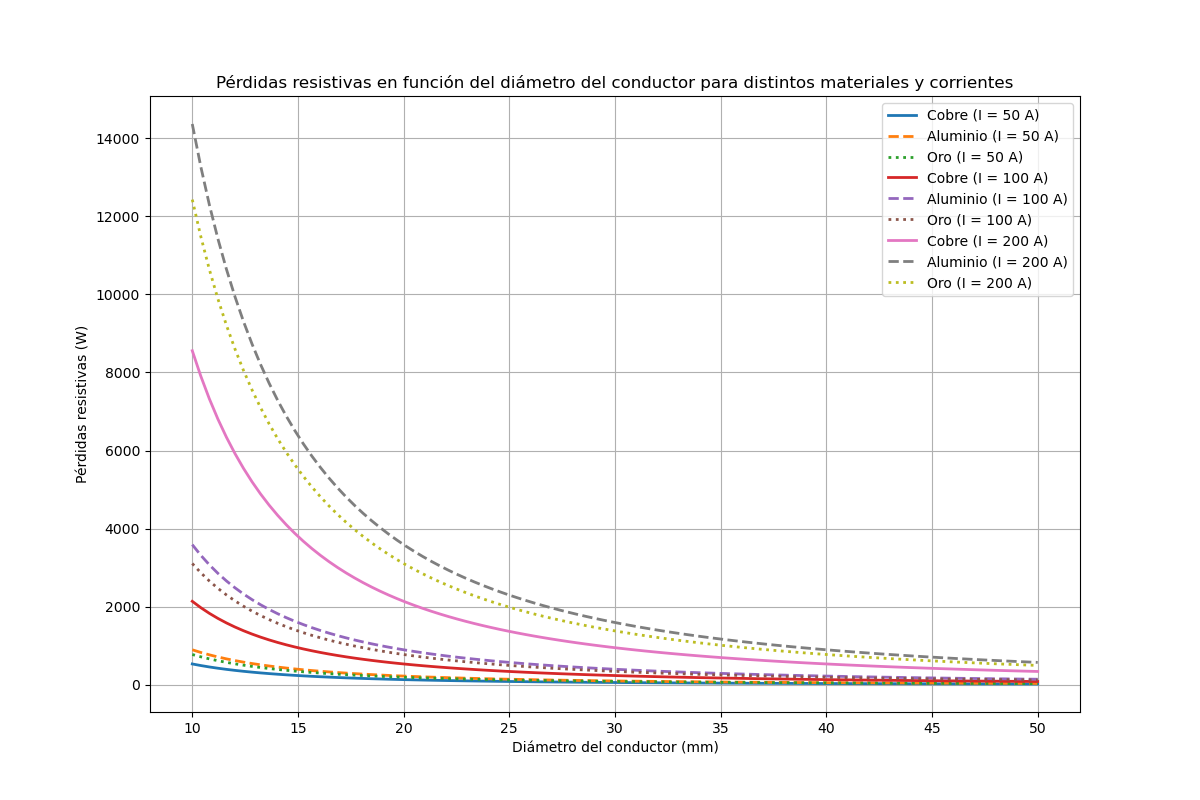
\includegraphics[width=\textwidth]{imagenes/perdidas_resistivas.png}
            \caption{Pérdidas resistivas en función del diámetro del conductor para distintos materiales y corrientes}
            \label{fig:Perdidas_resistivas}
        \end{figure}

       \begin{figure}[H]
           \centering
           \setcounter{figure}{0}
           \renewcommand{\figurename}{Tabla}
           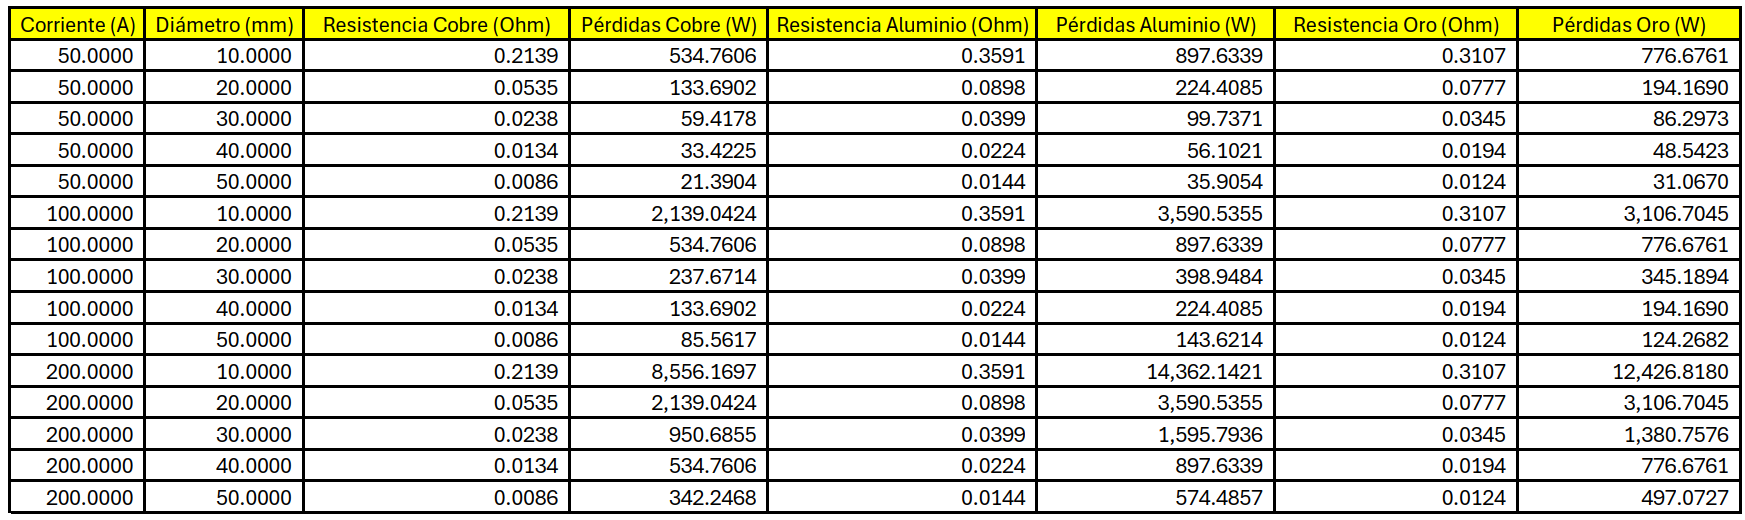
\includegraphics[width=\textwidth]{imagenes/sim_datos_perdidas.png}
           \caption{Tabla de datos de la simulación de Pérdidas resistivas en función del diámetro del conductor para distintos materiales y corrientes}
           \label{fig:sim_datos_perdidas}
       \end{figure}

      Cómo se puede apreciar en la Gráfica \ref{fig:Perdidas_resistivas} y la  Tabla \ref{fig:sim_datos_perdidas}, existe unas diferencias notables, en especial en la Gráfica \ref{fig:Perdidas_resistivas}, evidenciando a simple vista que los diferentes tipos de materiales si son importantes para la mitigación de las pérdidas resistivas del conductor. 

      Por otro lado, los distintos cambios realizado a los parámetros como lo fue la corriente, y su diámetro, trae como consecuencia la acción de aumentar o disminuir las pérdidas; seguidamente sus valores de resistencia, calculado indirectamente debido a los cambios antes efectuado, por ende, se obtuvo una aproximación de ¿Cuál es el material que va a mitigar las perdidas resistivas?

      Como se observa en la figura \ref{fig:awg}, los estándares en calibres van de 0.3606 (mm) a 11.86 (mm), es decir, se hará un énfasis a los valores de la tabla \ref{fig:sim_datos_perdidas}, que serán del 10 (mm) hasta los 30 (mm).

      Con una corriente de $50 \, A$, el cobre obtuvo una disminución con los distintos parámetros, observándose una disminución en sus resistencia y pérdidas, cuando su diámetro aumentaba, al igual que los demás elementos, sin embargo, de estos materiales quien le sigue la menor pérdida sería el oro, por ultimo el aluminio.

      Así mismo, va ocurriendo al aumentar la corriente, demostrando que existe mayor pérdida al tener mas corriente debido al movimiento de carga en el conductor, produciendo en este caso el efecto Joule.

      






\newpage